

%% Classe de documento
\documentclass[%% Opções (^ = padrão; > = para pacotes):
  a4paper,%% Tamanho de papel: a4paper, letterpaper (^), etc.
  12pt,%% Tamanho de fonte: 10pt (^), 11pt, 12pt, etc.
  fleqn,%% Alinhamento de equações à esquerda (centralizado por padrão)
%   draft,%% Aparência de documento (>): draft ou final (^)
  english,%% Idioma secundário (penúltimo) (>)
  brazilian,%% Idioma primário (último) (>)
]{article}
% \documentclass{scrartcl}
\usepackage[overload]{textcase} 

%% Pacotes utilizados
\usepackage[%% Opções (^ = padrão; ¹ = Leiaute A; ² = Leiaute B):
%   Layout    = A,%% Leiaute (margens): A (esquerda menor + recuo) ou B (iguais) (^)
%   Font      = Calibri,%% Fonte principal: Arial (²), Calibri (¹), Times ou LaTeX
%   RuleWidth = Text,%% Largura de linha (cabeçalho e rodapé): Zero (²), Text ou Paper (¹)
%   AffilIcon = Off,%% Ícones de e-mail, Lattes, ORCID e Instituição: On (^) ou Off
%   DocLic    = None,%% Licença do documento: CC (Creative Commons) (^) ou None
%   CCLic     = BY-NC-ND,%% Licença CC: BY (^), BY-SA, BY-ND, BY-NC, BY-NC-SA ou BY-NC-ND
%   Link      = TextColor,%% Cor de hyperlinks: DarkBlue (^) ou TextColor
%   PageNum   = Off,%% Numeração de páginas: On (^) ou Off
%   SectNum   = Off,%% Numeração de seções (\section): On (²) ou Off (¹)
%   SectUnnum = Center,%% Alinhamento de seções (\section*): Center (¹) ou Left (²)
%   Caption   = Left,%% Alinhamento de legendas: Center (^) ou Left
%   Source    = Left,%% Alinhamento de fonte (referência): Center (^) ou Left
%   ABNTCit   = NSB,%% Citação ABNT: AAY (NOME, ANO) (^), NRB (1) ou NSB [1]
%   BibDOI    = Icon,%% Ícone de DOI em referências: Icon ou Name (^)
%   BibURL    = Icon,%% Ícone de URL em referências: Icon ou URL (^)
]{utfpr-article}
\usepackage[hyperlink]{qrcode}
\usepackage{environ}
\usepackage[fleqn]{nccmath}
\usepackage{bm}
\usepackage{listings}
\NewEnviron{ceqnaling}
    {\vspace{3mm}
    \begin{ceqn}
        \begin{align*}
            \BODY
        \end{align*}
\end{ceqn}}
\usepackage{tikz}
\usetikzlibrary{chains}

\makeatletter
\DeclareRobustCommand{\rvdots}{%
  \vbox{
    \baselineskip4\p@\lineskiplimit\z@
    \kern-\p@
    \hbox{.}\hbox{.}\hbox{.}
  }}
\makeatother

\tikzset{
block/.style = {draw, minimum height=12mm, minimum width=26mm},
tmp/.style  = {coordinate}, 
sumpm/.style= {circle, draw, minimum size=9mm,
                append after command={\pgfextra{\let\LN\tikzlastnode}
                       (\LN.north west) edge (\LN.south east)
                            (\LN.south west) edge (\LN.north east)
                    node[left]     at (\LN.center) {$+$}
                    node[below]    at (\LN.center) {$-$}}},
sumpp/.style= {circle, draw, minimum size=9mm,
                append after command={\pgfextra{\let\LN\tikzlastnode}
                       (\LN.north west) edge (\LN.south east)
                            (\LN.south west) edge (\LN.north east)
                    node[left]     at (\LN.center) {$+$}
                    node[below]    at (\LN.center) {$+$}}},
input/.style = {coordinate},
output/.style= {coordinate},
pinstyle/.style = {pin edge={to-,thin,black}
}
}
\tikzstyle{sum} = [draw, fill=white, circle, node distance=1cm]

\newcommand{\Laplace}{\mathscr{L}}
\newcommand{\bN}{\mathbb Z_{\ge 0}}
\newcommand{\bPo}{\mathbb Z_{> 0}}
\newcommand{\bC}{\mathbb C}
\newcommand{\bZ}{\mathbb Z}
\newcommand{\bR}{\mathbb R}
\newcommand{\ztrans}{\mathcal{Z}}
\newcommand{\parth}[1]{\left(#1\right)}
\usepackage{enumerate}% http://ctan.org/pkg/enumerate
\usepackage{listings}
\lstdefinestyle{customc}{
  belowcaptionskip=1\baselineskip,
  breaklines=true,
  frame=L,
  xleftmargin=\parindent,
  language=C,
  showstringspaces=false,
  basicstyle=\footnotesize\ttfamily,
  keywordstyle=\bfseries\color{green!40!black},
  commentstyle=\itshape\color{purple!40!black},
  identifierstyle=\color{blue},
  stringstyle=\color{orange},
}

\lstdefinestyle{customasm}{
  belowcaptionskip=1\baselineskip,
  frame=L,
  xleftmargin=\parindent,
  language=[x86masm]Assembler,
  basicstyle=\footnotesize\ttfamily,
  commentstyle=\itshape\color{purple!40!black},
}

\lstset{escapechar=@,style=customc}
% \usepackage[shortlabels]{enumitem}
% \usepackage[ngerman]{babel} %Deutsche Sprachunterstützung
% \usepackage[utf8]{inputenc} %Umlaute
% \usepackage{subcaption}
% \usepackage{graphicx}
%%%% Autor(es) (de 1 a 8, Leiaute A; de 1 a 16, Leiaute B): {Número}; {Dados}
\Author{1}{%% Bolsista ou voluntário(a) principal (primeiro)
   Name        = {Danilo Gondo Chinen},%
   Email       = {nda@nda.com},%
 }
 \Author{2}{%% Bolsista ou voluntário(a) principal (primeiro)
   Name        = {Fabio Zhao Yuan Wang},%
   Email       = {fabioyuan@gmail.com},%
 }
 \Author{3}{%% Bolsista ou voluntário(a) principal (primeiro)
   Name        = {Gabriel Yudi Harada},%
   Email       = {acyrmarconato@gmail.com},%
 }
 \Author{4}{%% Bolsista ou voluntário(a) principal (primeiro)
   Name        = {Gregorio Antonio Daros Bussyguin},%
   Email       = {acyrmarconato@gmail.com},%
 }
% \Author{2}{%% Colaborador(a) (segundo ao penúltimo)
%   Name        = {Nome Completo do{(a)} Autor{(a)}-A2},%
%   Email       = {author2@domain},%
%   Lattes      = {0000000000000002},%% Opcional
%   ORCID       = {0000-0000-0000-0002},%% Opcional (CHKTEX 8)
%   Affiliation = {Instituição (Nome por Extenso), Cidade, Estado, País},%
%   Role        = {Discente de Nome do Curso},%% Leiaute B
% }
% \Author{3}{%% Orientador(a) principal (último)
%   Name        = {Nome Completo do{(a)} Autor{(a)}-A3},%
%   Email       = {author3@domain},%
%   Lattes      = {0000000000000003},%% Opcional
%   ORCID       = {0000-0000-0000-0003},%% Opcional (CHKTEX 8)
%   Affiliation = {\UTFPRName, Cidade, Paraná, Brasil},%
%   Role        = {Docente do Nome do Departamento ou Programa},%% Leiaute B
% }
%%%% Digital Object Identifier (DOI): {Name}
% \DOIName{10.1000/xyz123}
%%%% Datas: [Ano] (atual por padrão; opcional); {Recebido}; {Aprovado}
% \Dates[2023]{DD mmm. \YearNum}{DD mmm. \YearNum}
%%%% Evento (SEI, SICITE, etc.): {Dados}
% \EventInfo{%
%   Name    = {Nome Completo do Evento},%
%   Acronym = {EVNT \YearNum},%
%   Date    = {DD a DD de Mmmmmm de \YearNum},%
%   Local   = {Cidade, Paraná, Brasil},%
%   Logo    = {example-image},%% Arquivo de imagem em ./Logos/
%   Header  = {example-image},%% Arquivo de imagem em ./Headers/
%   URL     = {https://www.example.com/},%
% }
%%%% Instituição (se nenhum evento): {Dados}
 \InstitutionInfo{%
   Campus     = {Curitiba},%
   Department = {DAELN-Departamento de Eletrônica},%
 }
\usepackage{multirow}

%% Arquivo(s) de referências
\addbibresource{utfpr-article.bib}

%% Início do documento
\begin{document}
%introdução
\section{\NoCaseChange{Título e codinome do projeto}}
Processador de efeitos digital para instrumentos musicais
\section{\NoCaseChange{Link para o blog do projeto}}
O blog para o projeto está disponível no \href{https://www.notion.so/Introdu-o-2574e26b01868046a879e09b697b6f35?source=copy_link}{\textbf{aqui}}, no Notion.
\section{\NoCaseChange{Equipe}}
Danilo Gondo Chinen,
Fabio Zhao Yuan Wang,
Gabriel Yudi Harada,
Gregorio Antonio Daros Bussyguin
\section{\NoCaseChange{Declaração do escopo de alto nível:}}
O objetivo do projeto é desenvolver um processador de efeitos digital aplicável em instrumentos musicais, que será uma alternativa mais barata àquelas presentes no mercado. Além disso, o desenvolvimento próprio do equipamento permite maior flexibilidade em sua personalização, permitindo alterações sonoras que atinjam mais nichos presentes no mercado.

A solução também contará com uma interface de usuário, que, muitas vezes, não se faz presente em alternativas do mercado nessa faixa de preço. Dessa forma, será possível tornar o uso do processador mais intuitivo, a interface será implementada através de um aplicativo de dispositivo móvel e uma interface física com uma possibilidade de visualização de parâmetros, onde será possível selecionar efeitos, alterar parâmetros específicos e adicionar controles inteligentes. Além disso, a existência de um aplicativo torna o uso do produto mais cômodo, uma vez que não será estritamente necessário realizar as configurações diretamente no equipamento.
\begin{center}
\begin{tikzpicture}[auto, node distance=2cm, 
    start chain=going below]
    
    % \node [input, name=md] (midi) {};
    \node [block, name=mcu] (mcu) {MCU};
    \node [input, name=mcint, below of=mcu, node distance=6mm] (mcint) {};
    \node [input, name=mcurgt, right of=mcint, node distance=2mm] (mcurgt) {};
    \node [input, name=mcur2, right of=mcurgt, node distance=2mm] (mcur2) {};
    
    \node [input, name=mculft, left of=mcurgt, node distance=4mm] (mculft) {};
    \node [input, name=mcul2, left of=mculft, node distance=2mm] (mcul2) {};
    \node [input, name=mcul3, left of=mcul2, node distance=2mm] (mcul3) {};
    
    \node [block, below of=mcu,  name=spin] (spin) {Processador + ADC + DAC};
    \node [input, name=spinrgt,  below of=mcurgt, node distance=0.8cm] (spinrgt) {};
    \node [input, name=spinr2, right of=spinrgt, node distance=2mm] (spinr2) {};
    
    \node [input, name=spinlft, left of=spinrgt, node distance=4mm] (spinlft) {};
    \node [input, name=spinl2, left of=spinlft, node distance=2mm] (spinl2) {};
    \node [input, name=spinl3, left of=spinl2, node distance=2mm] (spinl3) {};

    
    \draw [->] (mcu) -- node [name=mcu2spin] {} (spin);
    \draw [->] (mcurgt) -- node {} (spinrgt);
    \draw [->] (mculft) -- node {} (spinlft);
    \draw [->] (mcul2) -- node {} (spinl2);
    \draw [->] (mcur2) -- node {} (spinr2);
    
    \draw [->] (mcul3) -- node {} (spinl3);

    \node [block, name=insig, left of=spin, node distance=60mm] (insig) 
    {Entrada Sinal (stereo)};
    \node [block, name=outsig, right of=spin, node distance=60mm] (outsig) {Saída Sinal (stereo)};

    \draw [->] (insig) -- node {} (spin);
    \draw [->] (spin) -- node {} (outsig);

    \node [block, name=apl, above of=mcu] (apl) {Aplicação};
    \node [input, name=apl2by, above of=apl] (apl2by) {};
    \node [block, name=bypass, right of=apl2by] (bypass) {Bypass};

    \draw[<->] (apl) -- node {} (mcu);

    \node [input, name=in_midi, left of=apl, node distance=40mm] 
    (in_midi) {MIDI in};
    \draw [->] (in_midi) -- node {MIDI in} (apl);


    \draw [dashed] (insig) |- (bypass);
    \draw [dashed] (outsig) |- (bypass);
    \draw [->] (mcu) -| (bypass);
        
    % \node [input, name=f2, below of=f1, node distance=9mm] 
    % (f2) {};
    
    % \node [block, right of=f1, node distance=4cm] (hi1) {$h_{i,1}[n]$};
    % \node [block, below of=hi1, node distance=9mm] (hi2) {$h_{i,2}[n]$};
    % \node [on chain, join, below of=hi2, 
    % node distance=9mm] (dotblock) {\rvdots};
    % \node [block, below of=dotblock, node distance=9mm] (hin_1) {$h_{i,(N_e-1)}[n]$};
    % \node [block, below of=hin_1, node distance=9mm] (hin) {$h_{i,N_e}[n]$};
    
    % \draw [->] (f1) -- node{$f_1[n]$} (hi1);    
    % \draw [->] (f2) -- node [name=f2k] {$f_2[n]$} (hi2);

    % \node [on chain, below of=f2k, 
    % node distance=-10mm] (dotfs) {\rvdots};
    % \node [input, name=fn_1, below of=f2, node distance=18mm] 
    % (fn_1) {};
    % \draw [->] (fn_1) -- node{$f_{N_e-1}[n]$} (hin_1);

    % \node [input, name=fn, below of=fn_1, node distance=9mm] (fn) {};
    % \draw [->] (fn) -- node{$f_{N_e}[n]$} (hin);


    % \node[input, name=hi1n, right of=hi1, node distance=13mm] (hi1n){};
    % \node[input, name=hi2n, below of=hi1n, node distance=9mm] (hi2n){};
    % \node[input, name=hin_1n, below of=hi2n, node distance=18mm] (hin_1n){};
    % \node[input, name=hinn, below of=hin_1n, node distance=9mm] (hinn){};

    
    % \node [sum, name=sum1, right of=dotblock, node distance = 2.5cm](sum1){$+$};

    % \draw [->] (hi1n) -- node{} (sum1);    
    % \draw [->] (hi2n) -- node{} (sum1);

    % \draw [->] (hin_1n) -- node{} (sum1);    
    % \draw [->] (hinn) -- node{} (sum1);

    % \node[output, name=gi, right of=sum1](gi){};
    % \draw [->] (sum1) -- node{$g_i[n]$} (gi);
    
    
\end{tikzpicture}
\end{center}
\\

\section{\NoCaseChange{Requisitos funcionais:}}

\subsection{\NoCaseChange{RF001 - Aplicação de Efeitos}}

Este requisito estabelece que o processador de efeitos digitais deve ser capaz de processar o sinal de áudio de um instrumento musical e aplicar uma gama variada de efeitos. Isso inclui, mas não se limita a, efeitos de modulação (chorus, flanger, phaser), delay (echo, reverb), distorção (overdrive, fuzz), e filtros (wah, equalizador). A implementação deve garantir que a qualidade do áudio não seja comprometida (com distorção e ruído, por exemplo) e que os efeitos sejam aplicados de forma transparente.

\subsection{\NoCaseChange{RF002 - Personalização de Efeitos}}

Para atender à demanda por flexibilidade e personalização, o sistema deve permitir que os usuários ajustem os parâmetros de cada efeito individualmente. Isso significa que, para um efeito de delay, por exemplo, o usuário poderá controlar o tempo de repetição, a realimentação e o nível de mixagem. Essa capacidade de personalização é crucial para que o produto se adapte a diferentes de usuários, permitindo a criação de sons que atendam a nichos específicos do mercado.

\subsection{\NoCaseChange{RF003 - Seleção de Efeitos (Aplicativo Móvel)}}

O aplicativo móvel servirá como uma interface para a interação do usuário com o processador de efeitos, o mesmo deve apresentar uma interface intuitiva, com ícones e nomes que representem fielmente a função de cada controlador para cada efeito.

\subsection{\NoCaseChange{RF004 - Alteração de Parâmetros (Aplicativo Móvel)}}

Complementando o RF003, o aplicativo móvel deve fornecer controles visuais (como sliders, botões e caixas de seleção) para que o usuário possa ajustar os parâmetros de cada efeito em tempo real. As alterações feitas no aplicativo devem ser imediatamente refletidas no processador de efeitos, permitindo ajuste fino.

\subsection{\NoCaseChange{RF005 - Visualização de Parâmetros (Aplicativo Móvel)}}

Para garantir que o usuário tenha total controle e feedback sobre as configurações do processador, o aplicativo móvel deve exibir de forma clara e em tempo real os valores atuais de todos os parâmetros dos efeitos ativos. Isso pode ser feito através de indicadores numéricos, gráficos ou medidores visuais, garantindo que o usuário sempre saiba o estado atual do seu equipamento.

\subsection{\NoCaseChange{RF006 - Seleção de Efeitos (Física)}}

Além da interface móvel, o processador de efeitos possuirá uma interface física que permita a seleção de efeitos diretamente no equipamento. Isso é importante para situações onde o uso do aplicativo móvel não é conveniente ou possível. A interface física pode incluir botões, pedais ou um dial rotativo para navegar entre os efeitos disponíveis.

\subsection{\NoCaseChange{RF007 - Alteração de Parâmetros (Física)}}

Similar ao RF004, a interface física deve permitir a alteração de parâmetros específicos dos efeitos. Isso pode ser implementado através de knobs, botões ou um display com menus interativos. A capacidade de ajustar parâmetros diretamente no equipamento oferece uma alternativa prática para ajustes rápidos durante uma performance ou ensaio.

\subsection{\NoCaseChange{RF008 - Visualização de Parâmetros (Física)}}

Para complementar o RF008, a interface física deve incluir um display  que mostre os parâmetros atuais dos efeitos. Isso permite que o usuário visualize as configurações sem a necessidade de consultar o aplicativo móvel, tornando a operação do equipamento mais autônoma e eficiente.

\subsection{\NoCaseChange{RF009 - Conectividade com Aplicativo Móvel}}

O processador de efeitos deve estabelecer uma conexão robusta e confiável com o aplicativo móvel, via Bluetooth. Essa conexão permitirá a troca bidirecional de dados, incluindo comandos do aplicativo para o processador e informações de status do processador para o aplicativo. 


\section{\NoCaseChange{Requisitos não funcionais:}}

\subsection{\NoCaseChange{RNF001 - Latência}}

Para instrumentos musicais, uma latência perceptível pode prejudicar a performance do músico, tornando a experiência antinatural e desconfortável. O objetivo é que a latência seja mínima, idealmente imperceptível ao ouvido humano, garantindo uma resposta imediata do efeito ao toque do instrumento. Implicando na escolha de algoritmos de processamento eficientes/otimizados.

\subsection{\NoCaseChange{RNF002 - Intuitividade}}

Tanto o aplicativo móvel quanto a interface física devem ser projetados de forma a permitir que o usuário compreenda e utilize as funcionalidades do processador de efeitos sem Dificuldade, envolvendo um design limpo, feedback visual claro e uma navegação lógica entre as opções.

\subsection{\NoCaseChange{RNF003 - Personalização Sonora}}

Além da simples alteração de parâmetros, engloba a arquitetura do sistema, que deve ser flexível o suficiente para permitir a adição de novos efeitos, a combinação de efeitos de maneiras inovadoras e a criação de cadeias de sinal complexas. O objetivo é que o processador não seja apenas um conjunto de efeitos, mas também uma plataforma que permita a experimentação sonora.

\subsection{\NoCaseChange{RNF004 - Estabilidade}}

O processador de efeitos deve operar de forma consistente, sem travamentos, falhas de áudio, desconexões inesperadas do aplicativo móvel ou comportamento errático dos efeitos. A robustez do hardware e a ausência de bugs críticos no software são essenciais para garantir a estabilidade.

\subsection{\NoCaseChange{RNF005 - Facilidade de Manutenção}}

Um design modular, tanto no hardware quanto no software, pode contribuir significativamente para a facilidade na manutenção. A capacidade de realizar atualizações de firmware remotamente (via aplicativo móvel, por exemplo) e a documentação clara do código e do hardware são aspectos importantes para garantir que o produto possa evoluir e ser mantido ao longo do tempo, prolongando sua vida útil e reduzindo os custos de suporte.


\section{\NoCaseChange{Anti requisitos}}
\begin{enumerate}
    \item O dispositivo não oferecerá a funcionalidade de afinador;
    \item O aplicativo será limitado à configuração dos parâmetros do pedal. Não será possível transmitir áudio ao aplicativo.
\end{enumerate}

\section{\NoCaseChange{Integração}}
Para o desenvolvimento do projeto, serão necessários conhecimentos nas áreas de programação em baixo nível (assembly), processamento de sinais, telecomunicações, sistemas microcontrolados e desenvolvimento de aplicações mobile. Em termos mais específicos, as principais matérias utilizadas neste projeto foram:

\begin{itemize}
  \item Fundamentos de programação
  \item Sistemas microcontrolados
  \item Análise e Projeto de sistemas
  \item Oficina de Integração 1
  \item Comunicação de Dados
\end{itemize}

\section{\NoCaseChange{Análise de Riscos}}
A tabela a seguir fornece o gerenciamento de riscos do projeto. Aspectos da solução como a latência de resposta entre os microcontroladores e integração das partes são as características mais críticas.

\begin{tabular}{ |p{3cm}||p{3cm}|p{3cm}|p{3cm}|  }
 \hline
 \multicolumn{4}{|c|}{Análise de riscos} \\
 \hline
 Problema& Probabilidade &Gravidade&Produto\\
 \hline
 Sobrecarga do microcontrolador     &  1    & 2     &   2\\
 Desistência de um integrante       &   1   & 2     &2\\
 Queima de componente               &3      & 2     &  6\\
 Latência entre dispositivos        &3      & 2     &  6\\
 Atraso na entrega de componentes   &   3   & 2     &6\\
 Ruído                              & 4     & 1     &4\\
 \hline
\end{tabular}

Em caso de sobrecarga do microcontrolador, a alternativa será a aquisição de um dispositivo mais potente, que seja capaz de atender às demandas. A desistência de um integrante acarretará maior carga de responsabilidades por parte dos membros restantes. A queima de um componente poderia atrasar o desenvolvimento do projeto, uma vez que seria necessário comprá-lo de volta. A latência entre dispositivos, bem como o ruído presente no sinal a ser modificado, podem ser amenizados com a realização extensiva de testes.

\section{\NoCaseChange{Cronograma detalhado}}
\href{https://docs.google.com/spreadsheets/d/1c_d0StAUM_7glkmwwl08T_zYdrpWEBFJgYbtEp_j8_Y/edit?gid=0#gid=0}{Disponível aqui.}

\section{\NoCaseChange{Materiais e métodos}}

Esta seção descreve os componentes de hardware e as tecnologias de software empregadas no desenvolvimento do processador de efeitos digitais . A arquitetura do sistema foi concebida para otimizar o desempenho, a flexibilidade e a relação custo-benefício e pode ser consultada no diagrama de blocos desenvolvido anteriormente.

\subsection{\NoCaseChange{Circuito Analógico}}

Este circuito é projetado para processar o sinal do instrumento, adequando-o para o processador FV-1 e um caminho de 'blend' para misturar o sinal original com o sinal processado. O circuito começa com a entrada do sinal da guitarra (IN), que passa por um estágio de buffer (U1) para garantir uma impedância de entrada adequada e evitar o carregamento da fonte do sinal. 

Após o estágio de buffer, o sinal é direcionado para o processador FV1. O sinal de entrada para o DSP é condicionado por dois filtros como C2, R3 e C3, enquanto o sinal de saída do DSP (OUT_DSP) é condicionado por C4, R4 e C5 antes de ser enviado para os estágios subsequentes, ambos os circuitos funcionando como filtros passa baixo.

Um aspecto fundamental deste circuito é o caminho de 'blend'. Este caminho permite que uma porção do sinal original (não processado pelo DSP) seja misturada com o sinal processado. No diagrama, o caminho 'BLEND' é visível, conectando-se antes do estágio de mistura final. Isso é essencial para pedais de efeitos que desejam preservar a clareza e o ataque do sinal original, enquanto adicionam o efeito do DSP. A mistura é realizada através de resistores (R5, R8, R7, R9) que combinam o sinal do caminho 'BLEND' com o sinal vindo do DSP (após U6 e C7).

Além de um circuito que controla o volume do sinal de saída para o efeito, pretendem-se adicionar um controle de filtro (garantindo maior usabilidade com diferentes faixas de sinal) e também uma saída balanceada, para conectar o processador em uma interface de audio.

\subsection{\NoCaseChange{Escolha de alimentação}}
Uma alimentação simétrica foi escolhida pois garante:

\begin{enumerate}
  \item Maior Slew Rate: Um op-amp com entradas de alimentação mais altas geralmente apresenta um slew rate (taxa de variação) maior. O slew rate descreve a velocidade com que a tensão de saída de um op-amp pode mudar em resposta a uma mudança imediata na tensão de entrada. Um slew rate mais alto permite que o op-amp reproduza com maior fidelidade sinais de guitarra mais rápidos (transientes) e harmônicos de alta frequência. Isso é particularmente importante para capturar a complexidade e a dinâmica do som da guitarra, especialmente após um estágio de distorção onde o sinal pode se tornar mais complexo e com transientes acentuados.

  \item Fidelidade na Reprodução de Sinais Distorcidos: Após o estágio de distorção, o sinal da guitarra pode conter formas de onda complexas e rápidas. O amplificador será alimentado com uma tensão de alimentação mais alta (utilizando uma fonte simétrica) para 
conseguir acompanhar a taxa rápida e as formas de onda complexas do sinal de guitarra mantendo a qualidade do áudio e evitando distorções indesejadas causadas pela limitação do slew rate do op-amp. 
\end{enumerate}
\begin{center}
  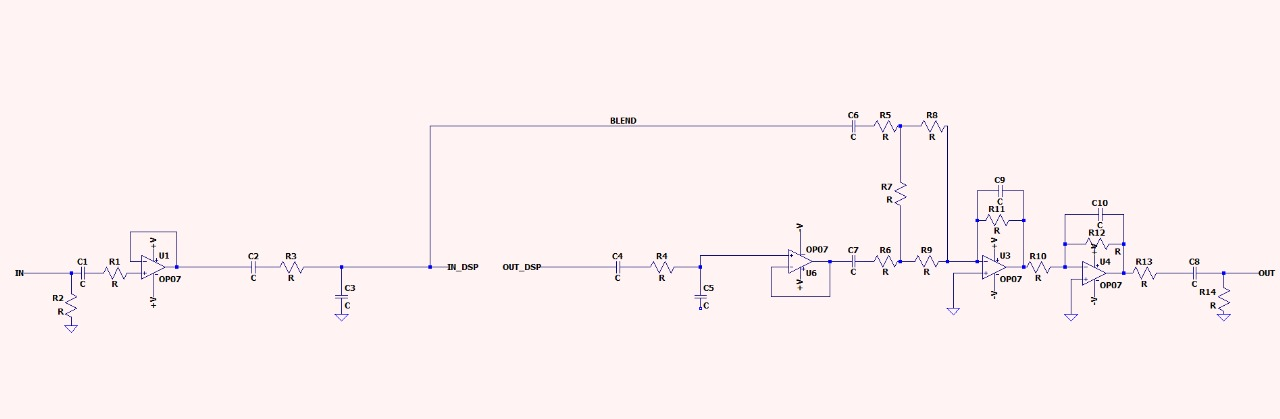
\includegraphics[width=16cm]{Diagrams/circ.png}
\end{center}

\subsection{\NoCaseChange{Hardware}}

\subsubsection{\NoCaseChange{Processador de Efeitos Spin FV-1}}

O coração do processamento de sinais de áudio neste projeto é o processador digital de sinais (DSP) Spin FV-1, fabricado pela Spin Semiconductor. Este circuito integrado (IC) é amplamente reconhecido na indústria de áudio, especialmente em pedais de efeitos de guitarra e sintetizadores, devido à sua capacidade de oferecer processamento de áudio de alta qualidade em um formato compacto e de baixo custo.

O FV-1 é um DSP estéreo que integra conversores analógico-digitais (ADCs) e digital-analógicos (DACs) de 24 bits, permitindo a entrada e saída de áudio diretamente sem a necessidade de componentes adicionais complexos para essa conversão. Ele opera a uma taxa de amostragem de 48 kHz e é capaz de executar 6 milhões de instruções por segundo (MIPS), o que é suficiente para a implementação de uma vasta gama de algoritmos de efeitos de áudio em tempo real.

Uma das características mais notáveis do FV-1 é sua flexibilidade de programação. O chip possui uma memória ROM interna com 8 programas de efeitos pré-carregados, como reverb, chorus e flanger. Além disso, ele pode acessar 8 programas adicionais a partir de uma EEPROM serial externa, o que permite aos desenvolvedores criar e carregar seus próprios algoritmos de efeitos personalizados. 

O FV-1 também inclui três entradas de potenciômetro, que podem ser utilizadas para controlar parâmetros dos efeitos em tempo real, como mixagem, tempo de decaimento ou intensidade. Isso facilita a integração com controles físicos na interface do usuário do pedal de efeitos. A programação do FV-1 é realizada em uma linguagem assembly específica, otimizada para o processamento de sinais digitais, conhecida como SpinASM. 

\subsubsection{\NoCaseChange{Microcontrolador}}

Um microcontrolador de propósito geral será empregado para gerenciar as diversas funcionalidades do processador de efeitos que não são diretamente relacionadas ao processamento de sinais de áudio, mas que são cruciais para a interação do usuário e a integração do sistema. A escolha de um microcontrolador adequado dependerá de requisitos específicos de conectividade (Bluetooth/Wi-Fi para a aplicação móvel), capacidade de processamento para lidar com a entrada MIDI e a complexidade do controle do FV-1, bem como a disponibilidade de periféricos como UART, SPI ou I2C para comunicação com outros componentes.

As principais funções atribuídas ao microcontrolador são:

\subsubsection{\NoCaseChange{Controle do Processador Spin FV-1}}

O microcontrolador atuará como a interface de controle principal para o processador Spin FV-1. Isso envolve o envio de comandos para selecionar programas de efeitos (tanto os internos quanto os carregados da EEPROM externa), ajustar os parâmetros dos efeitos através das entradas de potenciômetro do FV-1, e carregar novos programas de efeitos para a EEPROM. A comunicação entre o microcontrolador e o FV-1 será realizada através de protocolos de comunicação digital, garantindo a sincronização e o controle preciso dos efeitos.

\subsection{\NoCaseChange{Controle de Bypass de Efeitos}}

Para permitir que o sinal de áudio passe pelo processador de efeitos sem ser afetado pelos efeitos (modo bypass), o microcontrolador será responsável por gerenciar um circuito de by-pass que será implementado através de relés ou chaves eletrônicas que redirecionam o sinal de áudio diretamente da entrada para a saída, contornando o processador FV-1. O microcontrolador receberá comandos da interface física ou do aplicativo móvel para ativar ou desativar o modo bypass, proporcionando flexibilidade ao músico para alternar entre o som limpo do instrumento e o som com efeitos.

\subsubsection{\NoCaseChange{Gerenciamento da Entrada MIDI}}

O microcontrolador será encarregado de receber e interpretar mensagens MIDI, que podem incluir comandos para alterar programas de efeitos, ajustar parâmetros (via Control Change - CC), ou até mesmo sincronizar o tempo de efeitos baseados em tempo (via MIDI Clock). A implementação da entrada MIDI permitirá que o processador de efeitos seja integrado a setups musicais mais complexos, controlados por teclados MIDI, controladores ou estações de trabalho de áudio digital (DAWs).

\subsubsection{\NoCaseChange{Conectividade com a Aplicação Móvel}}

Uma das funcionalidades chave do projeto é a interface de usuário via aplicativo móvel. O microcontrolador será o ponto de conexão entre o hardware do processador de efeitos e o aplicativo. Isso implicará na implementação de um módulo de comunicação sem fio Bluetooth no microcontrolador, que enviará dados de status para o aplicativo e receberá comandos do aplicativo 

\subsection{\NoCaseChange{Software}}

As funcionalidades do processador de efeitos digitais serão implementadas através de uma arquitetura de software distribuída, abrangendo três camadas principais: a aplicação móvel para interação do usuário, o firmware do microcontrolador para controle de hardware e comunicação, e o código assembly para o processamento de sinais no FV-1.

\subsubsection{\NoCaseChange{Aplicação Móvel (JavaScript)}}

A interface de usuário para o processador de efeitos será desenvolvida como um aplicativo móvel, utilizando JavaScript. 

\begin{enumerate}
    \item Interface Gráfica: Fornecer uma interface intuitiva para seleção de efeitos, ajuste de parâmetros e configuração de controles inteligentes;
    \item Comunicação: Estabelecer e manter a comunicação sem fio com o microcontrolador (via Bluetooth ou Wi-Fi) para enviar comandos e receber dados de status;
    \item Visualização de Parâmetros: Exibir em tempo real os valores dos parâmetros dos efeitos ativos, proporcionando feedback visual ao usuário.

\end{enumerate}

\subsubsection{\NoCaseChange{Firmware do Microcontrolador (C)}}

O firmware do microcontrolador será desenvolvido em linguagem C num sistema embarcado, permitindo controle de baixo nível sobre o hardware. O código em C no microcontrolador será responsável por:

\begin{itemize}
    \item Controle do FV-1: Gerenciar a comunicação com o processador Spin FV-1, enviando comandos para seleção de programas e ajuste de parâmetros;
    \item Gerenciamento de Periféricos: Controlar os periféricos do microcontrolador, como GPIOs para o bypass de efeitos, interfaces de comunicação serial (UART, SPI, I2C) para interação com outros componentes e a interface MIDI;
    \item Processamento de Entrada MIDI: Interpretar as mensagens MIDI recebidas e traduzi-las em ações para o FV-1 ou para o próprio microcontrolador;
    \item Comunicação Sem Fio: Gerenciar o módulo de comunicação sem fio (Bluetooth/Wi-Fi) para interagir com o aplicativo móvel;
    \item Lógica de Controle: Implementar a lógica de controle geral do sistema, coordenando as interações entre a interface física, o FV-1 e o aplicativo móvel.

\end{itemize}

\subsubsection{\NoCaseChange{Programação do FV-1 (Assembly)}}

Os algoritmos de processamento de sinais digitais que serão executados diretamente no processador Spin FV-1 serão programados em linguagem assembly específica do FV-1 (SpinASM). Embora a programação em assembly seja mais complexa e de baixo nível, ela é essencial para otimizar o desempenho e a eficiência dos efeitos de áudio. A programação em assembly permite um controle preciso sobre os recursos do DSP, garantindo que os efeitos sejam executados com a menor latência possível e utilizando os recursos de hardware de forma otimizada. Isso é crucial para a criação de efeitos de áudio complexos e de alta qualidade que atendam aos requisitos de desempenho do projeto.

%link
% NOTHING

\end{document}
